% !TeX spellcheck = en_US
\section{Problem 12}

In order to evaluate the expression "\verb|not(A(x) OR B(x))|", we must first take a look at how fuzzy logic differs from binary logic at operation level.
In binary logic we have three basic operations: \verb*|AND(x,y)|, \verb*|OR(x,y)| and \verb*|NOT(x)|. But, in fuzzy logic, where a function can have a value in the range of $\left[0...1\right]$, things are slightly different.
The binary operation \verb*|AND(x,y)| is equivalent to \verb|MIN(x,y)| from fuzzy logic, \verb*|OR(x,y)| to \verb*|MAX(x,y)| and \verb*|NOT(x)| to \verb|1-x|.

\begin{wrapfigure}{R}{0.45\textwidth}
	\vspace{-0.5cm}
	\centering
	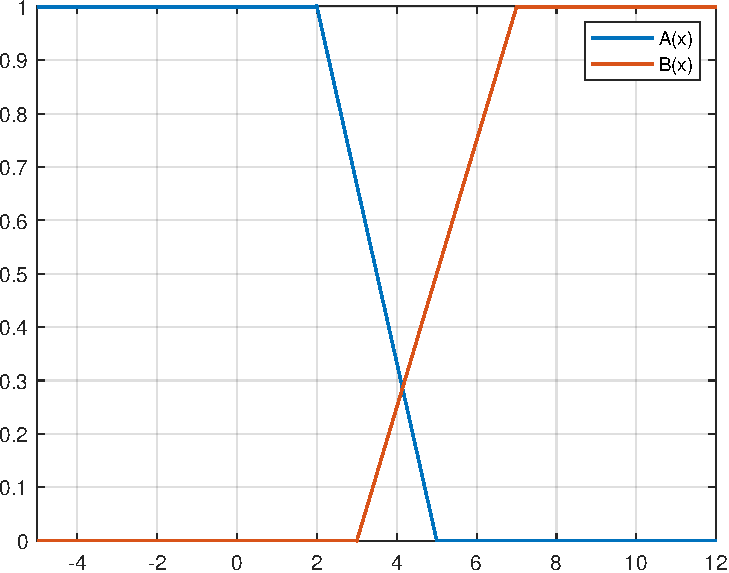
\includegraphics[width=0.4\textwidth]{../Problem 12/a_b_functions.pdf}
	\caption{Plot of A(x), B(x)}
	\label{fig:prob_12_a_b}
\end{wrapfigure}

We need to find the proper $x$ for which the previous expression has the maximum value. First, we calculate the expression and then find the correct $x$.
To achieve this, we need to divide our calculations into ranges. 

Starting for $x \le 2$, $"A(x) \text{ AND } B(x)"$ is equal to $"\textit{max}\left(A(x), B(x)\right)" = 1$. Applying De Morgan's law, we therefore have $\textit{max}\left(A(x), B(x)\right) \Rightarrow \textit{not}\left(A(x) \textit{ or } B(x)\right) = 0$.
Exactly the same result is obtained with $x \ge 7$.

Things are a bit different in $2 \le x \le 7$. The function $A(x)$ starts to fall while $B(x)$ starts to rise. The point at which the two functions cross is important for the definition of the required expression and can be obtained by solving the equation:
\[
A(x_{crit}) = B(x_{crit}) \Leftrightarrow 1 - \frac{x_{crit}-2}{3} = \frac{x_{crit}-3}{4} \Rightarrow x_{crit} = \frac{29}{7}
\]

For $2 \le x \le \frac{29}{7}$, $\textit{max}\left(A(x), B(x)\right) = 1 - \dfrac{x-2}{3} = A(x)$, because in this region $A(x)$ lies above $B(x)$. Thus, $\textit{not}\left(A(x) \textit{ or } B(x)\right) = \dfrac{x-2}{3}$.

Using the same logic, we find out that for $\frac{29}{7} \le x \le 7$, $\textit{not}\left(A(x) \textit{ or } B(x)\right) = 1 - \dfrac{x-3}{4}$. 

Therefore, the expression $f(x) = \textit{not}\left(A(x) \textit{ or } B(x)\right)$ is summarized below:
\begin{equation}
	f(x) = \left\{
	\begin{array}{cc}
		0 & x \le 2, \\[4mm]
		\dfrac{x-2}{3} & 2 \le x \le \frac{29}{7}, \\[4mm]
		1 - \dfrac{x-3}{4} & \frac{29}{7} \le x \le 7, \\[4mm]
		0 & x \ge 7\\
	\end{array}
	\right.
\end{equation}

By plotting this function in figure~\ref{fig:prob_12_expression_plot}, we can clearly see that the maximum occurs at $x = x_{crit} = \dfrac{29}{7}$ and its value is $0.715465$.

\begin{figure}[htp]
	\centering
	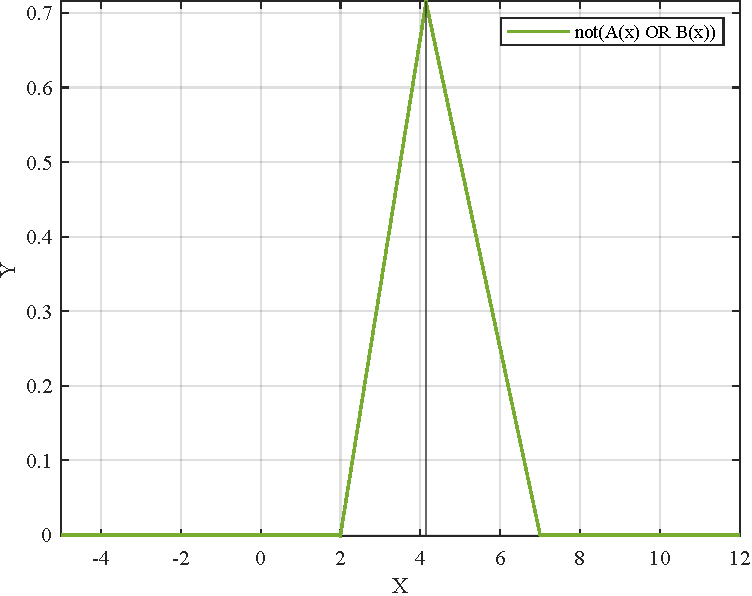
\includegraphics[width=.45\textwidth]{../Problem 12/expression_plot.pdf}
	\caption{Expression's plot}
	\label{fig:prob_12_expression_plot}
\end{figure}
